\documentclass{beamer}
\usepackage[francais]{babel}
\usepackage{graphicx}
\setbeamertemplate{items}[circle]
\usetheme{default}
%%\useoutertheme{infolines} 
\setbeamertemplate{footline}
{
  \leavevmode%
  \hbox{%
  \begin{beamercolorbox}[wd=.333333\paperwidth,ht=2.25ex,dp=1ex,center]{author in head/foot}%
    \usebeamerfont{author in head/foot}
  \end{beamercolorbox}%
  \begin{beamercolorbox}[wd=.333333\paperwidth,ht=2.25ex,dp=1ex,center]{title in head/foot}%
    \usebeamerfont{title in head/foot}\insertshorttitle
  \end{beamercolorbox}%
  \begin{beamercolorbox}[wd=.333333\paperwidth,ht=2.25ex,dp=1ex,right]{date in head/foot}%
    \usebeamerfont{date in head/foot}\insertshortdate{}\hspace*{2em}
    \insertframenumber{} / \inserttotalframenumber\hspace*{2ex} 
  \end{beamercolorbox}}%
  \vskip0pt%
}

\title{Projet MF Banking}
\setbeamertemplate{navigation symbols}{}
\author{K\'evin POGORZELSKI, Fran\c cois GUILLAIN, Tahar BAKIR\\ Bastien LEMALE, Guillaume VAROQUAUX et Pierre DAL-PRA}
\begin{document}

\begin{frame}
	\maketitle
\end{frame}

\begin{frame}{Plan}
	\begin{itemize}
		\item Pr\'esentation des fonctionnalit\'es impl\'ement\'ees (user stories) 
		\item Organisation du projet
			\begin{itemize}
				\item Management du travail
				\item Environnement de d\'eveloppement
			\end{itemize}
		\item Architecture du projet
			\begin{itemize}
				\item Objets du mod\`ele
				\item Organisation des modules
			\end{itemize}
		\item Pr\'esentation technique
			\begin{itemize}
				\item Back-office
				\item Front-office
				\item Tests (unitaires et d'int\'egration)
				\item Web Services
			\end{itemize}
	\end{itemize}
\end{frame}

\begin{frame}
	\begin{center}
		\huge{Pr\'esentation des fonctionnalit\'es impl\'ement\'ees (user stories) }
	\end{center}
\end{frame}

\begin{frame}{Sprint 0+1}
\begin{itemize}
	\item Mise en place de l'environnement de d\'eveloppement
	\item Consulter sur ma page d'accueil le solde de mes comptes esp\`ece
	\item Acc\'eder \`a ma page de login
	\item Me logger
	\item BONUS : Page admin basique
\end{itemize}
\end{frame}

\begin{frame}{Sprint 2}
\begin{itemize}
	\item Consulter le d\'etail d'un compte esp\`ece avec le d\'etail des op\'erations d'un mois donn\'e + d\'etail des op\'erations carte \`a part
	\item Consulter le d\'etail des op\'erations carte pour un mois donn\'e
\end{itemize}
\end{frame}

\begin{frame}{Sprint 3}
\begin{itemize}
	\item R\'ealiser des virements internes
	\item R\'ealiser des virements externes
	\item Exporter au format Excel le relev\'e des op\'erations pour un mois donn\'e
	\item Consulter l'historique de mes virements
	\item Consulter sur ma page d'accueil l'encours carte sur chacun de mes comptes esp\`ece
	\item Consulter sur ma page d'accueil le solde pr\'evisionnel de chacun de mes comptes esp\`ece
\end{itemize}
\end{frame}

\begin{frame}{Sprint 4}
\begin{itemize}
	\item Ajout de webservices REST et SOAP
	\item BONUS : Am\'elioration de la page admin
	\item BONUS : Mise \`a jour automatique du solde, du solde pr\'evisionnel et de l'encours carte 
\end{itemize}
\end{frame}


\begin{frame}
	\begin{center}
		\huge{Organisation du projet}
	\end{center}
\end{frame}

\begin{frame}{Management du travail}
	\begin{itemize}
		\item Gestion du projet selon la m\'ethode Scrum
		\item Part importante du projet r\'ealis\'ee en Pair Programming
		\item Polyvalence des d\'evloppeurs
	\end{itemize}
\end{frame}

\begin{frame}{Environnement de d\'eveloppement}
	\begin{itemize}
		\item Build : Maven
		\item Int\'egration continue : Jenkins $\rightarrow$ Build incassable
		\item SCM : Git
		\item Serveur : Tomcat
		\item Bases de donn\'ees : PostgreSQL, HSQLDB
	\end{itemize}
\end{frame}



\begin{frame}
	\begin{center}
		\huge{Architecture du projet}
	\end{center}
\end{frame}

\begin{frame}{Diagramme E/A}
	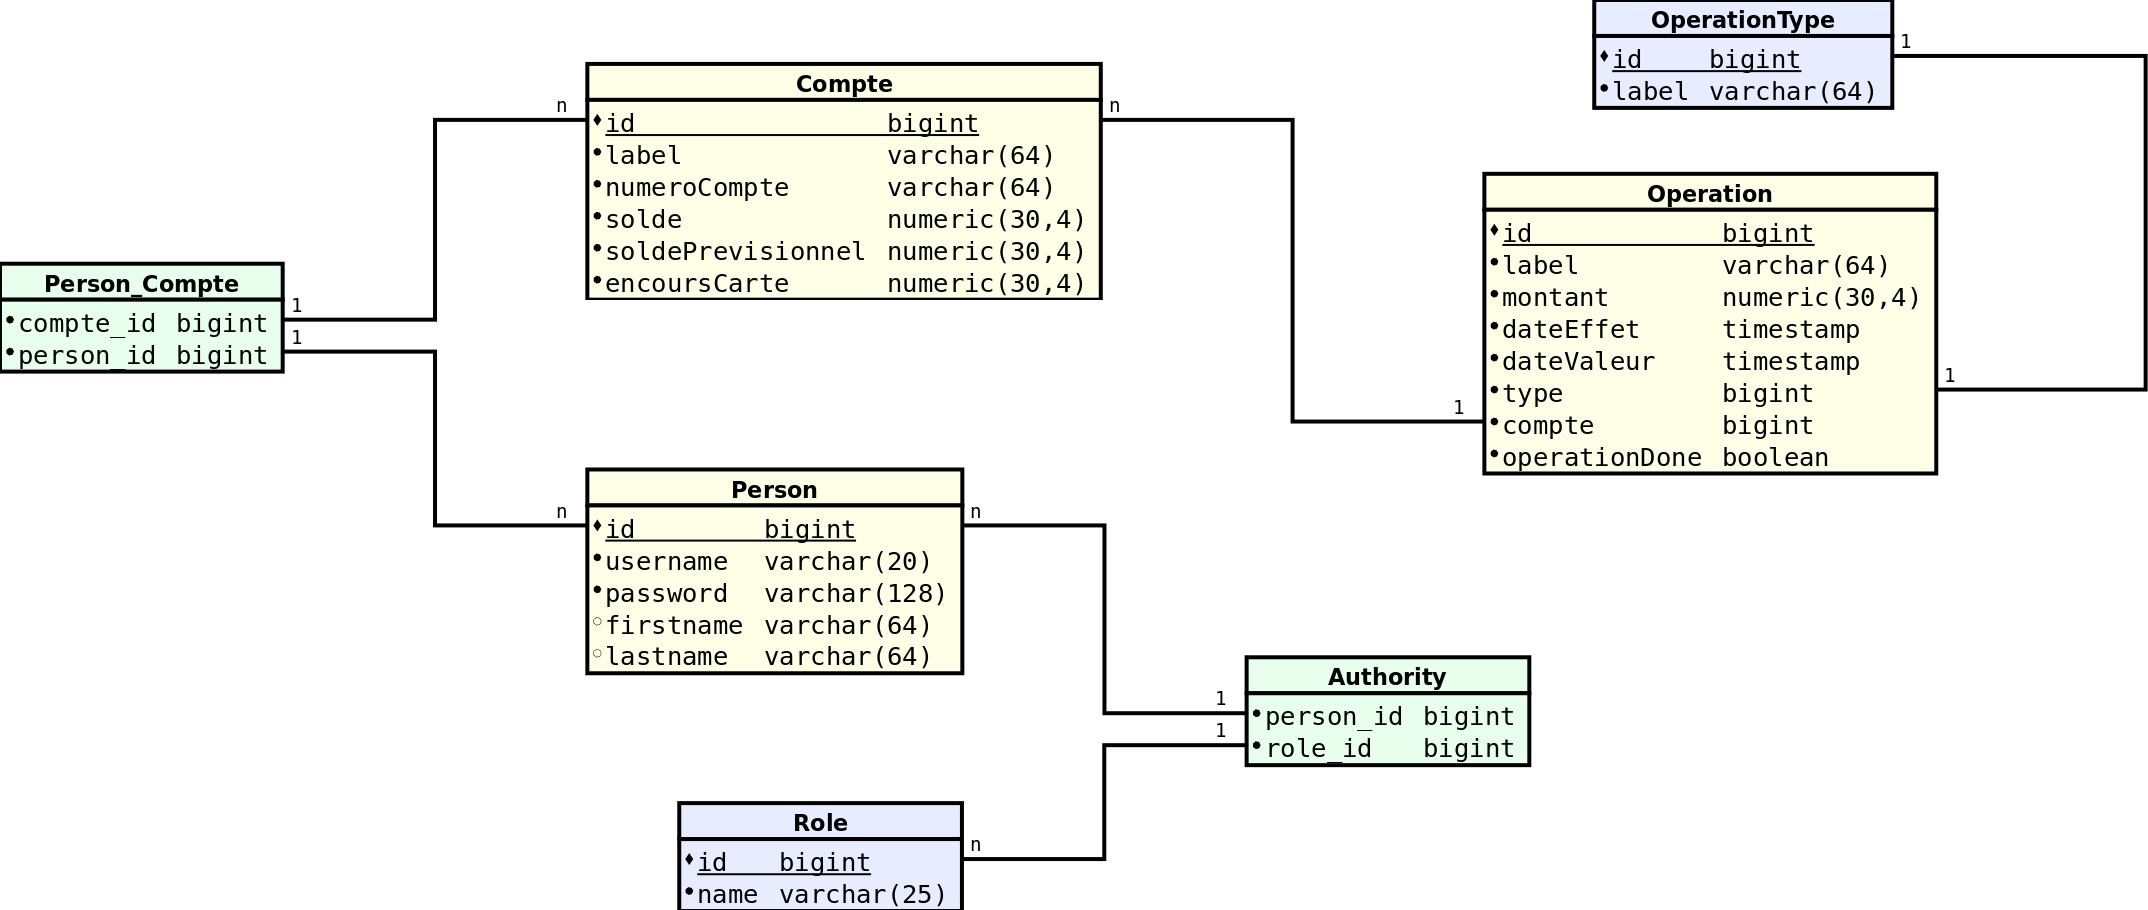
\includegraphics[scale=0.2]{diagramme_modele.png}
\end{frame}

\begin{frame}{Organisation des modules Maven du projet}
	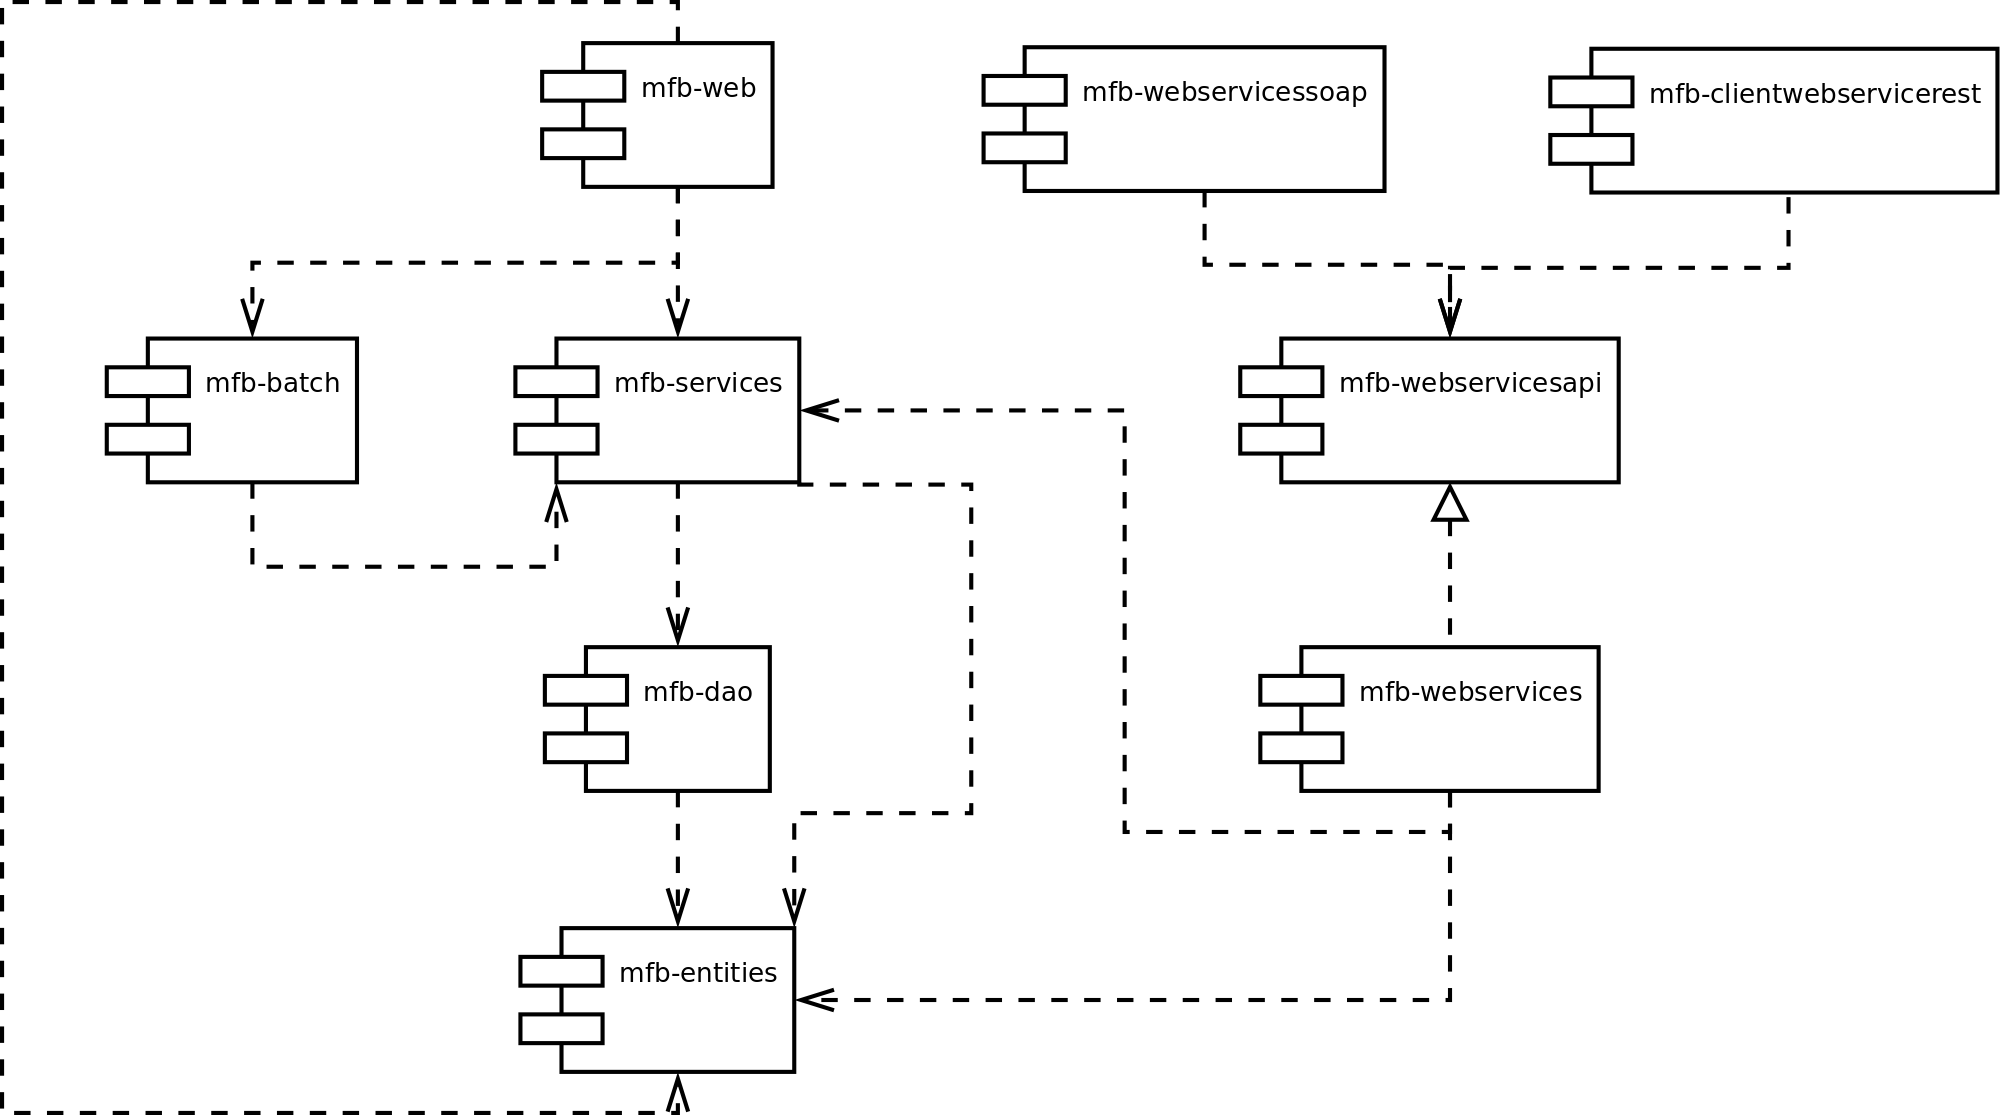
\includegraphics[scale=0.2]{diagramme_modules.png}
\end{frame}



\begin{frame}
	\begin{center}
		 \huge{Pr\'esentation technique}
	\end{center}
\end{frame}

\begin{frame}{Back-office}
	\begin{itemize}
		\item Spring (IOC, DB, TX, MVC,Validation\ldots) \& Spring Security
		\item Persistence
		\begin{itemize}
			\item ORM : Hibernate + JPA 
			\item Versionnement des sch\'emas : Liquibase
			\item Pool de connexion : Tomcat JDBC			
			\item Cache de 2nd niveau: Ehcache
		\end{itemize}
		\item Spring Batch
		\item Logging : SLF4J \& Logback
	\end{itemize}
\end{frame}

\begin{frame}{Front-office}	
	\begin{itemize}
		\item Internationalisation (Spring)
		\item Apache Tiles
		\item Twitter Bootstrap
		\item Apache POI
	\end{itemize}
\end{frame}

\begin{frame}{Tests}
	\begin{itemize}
		\item Tests unitaires : 
			\begin{itemize}
				\item Junit
				\item DBUnit (via spring-db-unit)
				\item Mockito
			\end{itemize}
		\item Tests d'int\'egration $\rightarrow$ Selenium :
			\begin{itemize}
				\item Int\'egration \`a Maven
				\item D\'eploiement sur un serveur Jetty
				\item Utilise une base PostgreSQL de test (remplie/vid\'ee \`a chaque test), suite \`a des probl\`emes avec HSQLDB
			\end{itemize}
	\end{itemize}
\end{frame}

\begin{frame}{Web Services}
	\begin{itemize}
		\item Apache CXF
		\begin{itemize}
			\item SOAP
			\item REST (JSON, via Jackson)
		\end{itemize}
	\end{itemize}
\end{frame}

\end{document}
